% !TEX encoding = UTF-8 Unicode
% !TEX TS-program = pdflatex
% !TEX root = ../Tesi.tex



%************************************************
\myChapter{Condizioni al contorno}
%************************************************

\label{cap:boundary}
\section{Interfaccia}
In questa sezione verranno brevemente riportate le classiche condizioni di interfaccia associate al problema elettro-magnetico. 
Maggiori dettagli possono essere trovati in \citep{zaglmayr_high_2006} o \citep{markus_zahn_electromagnetic_????}.
 
Si assuma un dominio $V \in \TTTT{R}^3$ suddiviso nelle due parti $V_1$ e $V_2$ in modo che $V = V_1 \cup V_2$. Si indichino con il simbolo $\partial\left(\right)$ le superfici al contorno dei diversi domini e si definisca e $\Gamma = \partial V_1 \cap \partial V_2$ (figura \ref{fig:4.7}).

\begin{SCfigure}[2.5][htp]
\centering
\caption{Domini arbitrari per la determinazione delle condizioni al contorno \eqref{eq:4interface_b3} e \eqref{eq:4interface_d3}}
\label{fig:4.7}
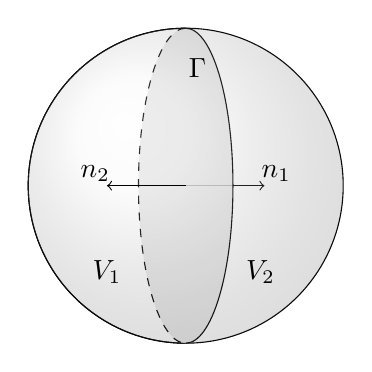
\begin{tikzpicture}
\draw[black] (0,0) circle (2);
\draw[black] (0,2) arc (90:270:2);
\draw[->] (0,0) -- (1,0);
\fill[black!10!white, opacity = .8] (0,0) ellipse (.6 and 2);
\draw[dashed] (0,2) arc (90:270:.6 and 2);
\draw (0,2) arc (450:270:.6 and 2);
\shade[ball color=black!10!white,opacity=0.20] (0,0) circle (2);

\draw[->] (0,0) -- (-1,0);
\draw (-1,-1.1) node {$V_1$}; %label
\draw (.95,-1.1) node {$V_2$}; %label
\draw (1.15,0.15) node {$\T{n_1}$}; %label
\draw (-1.15,0.15) node {$\T{n_2}$}; %label
\draw (.15,1.5) node {$\Gamma$}; %label
\end{tikzpicture}
\end{SCfigure}

Si applichi l'equazione \eqref{eq:2max4} al dominio $V$:
\begin{align}
\label{eq:4interface_b}
\int_{\partial V} \T{b}\cdot \T{n} ds &= 0\\
\int_{\partial V_1} \T{b_1}\cdot \T{n_1} ds &= 0\\
\int_{\partial V_2} \T{b_2}\cdot \T{n_2} ds &= 0.
\end{align}

Da cui
\begin{align}
\label{eq:4interface_b2}
0&=\int_{\partial V} \T{b}\cdot \T{n} ds\nonumber\\
&=\int_{\partial V_1} \T{b_1}\cdot \T{n_1} d\T{s}+\int_{\partial V_2} \T{b_2}\cdot \T{n_2} d\T{s}+\nonumber\\
&-\int_{\Gamma} \T{b_1}\cdot \T{n_1} d\T{s}-\int_{\Gamma} \T{b_2}\cdot \T{n_2} d\T{s}\nonumber\\
&= \int_\Gamma \Bigl\langle \T{b} \cdot \T{n} \Bigr\rangle ds,
\end{align}
dove
\[
\Bigl\langle u \Bigr\rangle = u_2 -u_1 
\]
e
\[
\Bigl\langle\T{v}\cdot \T{n}\Bigr\rangle = (\T{v}_2 -\T{v}_1)\cdot\T{n_2}. 
\]

Si ottiene quindi la condizione di interfaccia:
\begin{equation}
\label{eq:4interface_b3}
\Bigl\langle \T{b} \cdot \T{n} \Bigr\rangle = 0.
\end{equation}

Passaggi analoghi possono essere svolti per l'equazione \eqref{eq:2max2}. Si supponga, per generalità, di avere una distribuzione di carica elettrica $\rho$ nel volume e $\rho_s$ per la superficie. Si ha allora:
\begin{align}
\label{eq:4interface_d}
\int_{\partial V} \T{d}\cdot \T{n} ds &= \int_{V}\rho dv + \int_\Gamma \rho_s ds\nonumber\\ 
&=\int_{V_1}\rho dx+\int_{V_2}\rho dv+\int_\Gamma \rho_s ds\\
\label{eq:4interface_dbis}
\int_{\partial V_1} \T{d_1}\cdot \T{n_1} d\T{s} &= \int_{V_1}\rho dv\\
\label{eq:4interface_dtris}
\int_{\partial V_2} \T{d_2}\cdot \T{n_2} d\T{s} &= \int_{V_2}\rho dv.
\end{align}

Sottraendo i termini delle equazioni \eqref{eq:4interface_dbis} e \eqref{eq:4interface_dtris} alla \eqref{eq:4interface_d} si ottiene:
\begin{align}
\label{eq:4interface_d2}
\int_{\partial V-\partial V_1-\partial V_2}\T{d}\cdot\T{n} ds &= \int_\Gamma \rho_s ds\nonumber\\
-\int_\Gamma \T{d_1} \cdot \T{n_1} -\int_\Gamma \T{d_2} \cdot \T{n_2} &= \int_\Gamma \rho_s ds\nonumber\\
-\int_\Gamma \Bigl\langle\T{d} \cdot \T{n}\Bigr\rangle ds &=\int_\Gamma \rho_s ds,
\end{align}
da cui
\begin{equation}
\label{eq:4interface_d3}
\Bigl\langle \T{d} \cdot \T{n} \Bigr\rangle = -\rho_s.
\end{equation}

Proseguiamo cercando le condizioni di interfaccia per il campo $\T{e}$. Con riferimento alla figura \ref{fig:4.8} intersechiamo la superficie $\Gamma$ con il piano $\Delta$ in modo che $L = \Gamma \cap \Delta$ sia la linea d'intersezione fra le due superfici.

\begin{figure}[htp]
\centering
\caption{Domini arbitrari per la determinazione delle condizioni al contorno \eqref{eq:4interface_e3} e \eqref{eq:4interface_h}}
\label{fig:4.8}
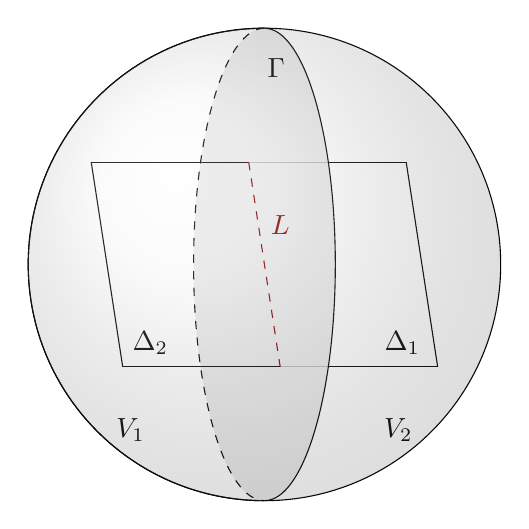
\begin{tikzpicture}
\draw (0,0) circle (3.);
\draw (0,3.) arc (90:270:3.);
\draw (1.8,1.3) -- (2.2,-1.3);
\draw (-2.2,1.3) -- (-1.8,-1.3);
\draw (1.8,1.3) -- (-.2,1.3);
\draw (2.2,-1.3) -- (.2,-1.3);
\fill[black!10!white, opacity = .8] (0,0) ellipse (.9 and 3);
\draw (-.2,1.3) -- (-2.2,1.3);
\draw (.2,-1.3) -- (-1.8,-1.3);
\draw[dashed] (0,3) arc (90:270:.9 and 3);
\draw (0,-3) arc (270:450:.9 and 3);
\draw[black!50!red,dashed] (-.2,1.3) -- (.2,-1.3);
\draw (-1.7,-2.1) node {$V_1$}; %label
\draw (1.7,-2.1) node {$V_2$}; %label
\draw (.15,2.5) node {$\Gamma$}; %label
\draw (1.75,-1.) node {$\Delta_1$}; %label
\draw (-1.45,-1.) node {$\Delta_2$}; %label
\draw[black!50!red,dashed] (0.2,0.5) node {$L$}; %label
\shade[ball color=black!10!white,opacity=0.20] (0,0) circle (3);
\end{tikzpicture}
\end{figure}

Applicando la legge di Faraday (\eqref{eq:2faraday}) ai domini $\Delta$, $\Delta_1$ e $\Delta_2$ si ha:
\begin{align}
\label{eq:4interface_e}
\int_{\partial \Delta} \T{e}\cdot \T{t} dl &= 0\\
\int_{\partial \Delta_1} \T{e_1}\cdot \T{t_1} dl &= 0\\
\int_{\partial \Delta_2} \T{e_2}\cdot \T{t_2} dl &= 0,
\end{align}
da cui
\begin{align}
\label{eq:4interface_e2}
\int_{\partial \Delta_1} \T{e1}\cdot \T{t1} dl + \int_{\partial \Delta_2} \T{e2}\cdot \T{t2} dl + &\nonumber\\
- \int_{L} \T{e_1}\cdot \T{t_1} dl - \int_{L} \T{e_2}\cdot \T{t_2} dl &= 0 \nonumber\\
- \int_{L} \T{e_1}\cdot \T{t_1} dl - \int_{L} T{e_2}\cdot \T{t_2} dl &= 0 \nonumber\\
- \int_{L} \left( \T{e_2}-\T{e_1}\right) \cdot \T{t_2} dl &= 0 \nonumber\\
- \int_{L} \Bigl\langle\T{e} \cdot \T{t} \Bigr\rangle dl &= 0.
\end{align}
Notando che l'equazione deve valere per qualsiasi orientazione del piano $\Delta$ (quindi per qualsiasi direzione del versore $\T{t}$ sulla curva $\Gamma$), si ottiene:
\begin{equation}
\label{eq:4interface_e3}
\Bigl\langle\T{e} \times \T{n} \Bigr\rangle = 0.
\end{equation}

Infine, analizzando l'equazione \eqref{eq:2ampere2} e ripercorrendo i passaggi appena svolti, si ottiene
\begin{equation}
\label{eq:4interface_h}
\Bigl\langle\T{h} \times \T{n} \Bigr\rangle = -\T{j_s},
\end{equation}
dove $\T{j_s}$ è l'eventuale corrente superficiale che percorre $\Gamma$.

Applichiamo ora le condizioni di interfaccia \eqref{eq:4interface_d3} e \eqref{eq:4interface_e3} nel caso in cui uno dei due materiali sia rappresentabile come \textit{PEC}. In tal caso l'intensità di campo elettrico è nulla nel materiale e si hanno le condizioni al contorno:
\begin{align}
\label{eq:4pec_d}
\left( \T{d} -\T{d_{PEC}}\right)\cdot \T{n} &= -\rho_s\nonumber\\
\T{d}\cdot \T{n} &= -\rho_s
\end{align}
e
\begin{align}
\label{eq:4pec_e}
\left( \T{e} -\T{e_{PEC}}\right)\times \T{n} &= 0\nonumber\\
\T{e}\times \T{n} &= 0.
\end{align}

Allo stesso modo possono essere trovate le condizioni al contorno per i conduttori magnetici perfetti:
\begin{align}
\label{eq:4pmc_b}
\left( \T{b} -\T{b_{PEC}}\right)\cdot \T{n} &= 0\nonumber\\
\T{b}\cdot \T{n} &= 0
\end{align}
e
\begin{align}
\label{eq:4pec_h}
\left( \T{h} -\T{h_{PEC}}\right) \times \T{n} &= -\T{j_s} \nonumber\\
\T{h} \times \T{n} &= -\T{j_s}.
\end{align}

Infine, per domini aperti si riportano le condizioni al contorno:
\begin{align}
\label{eq:4cond_inf}
\lim_{\T{x}\rightarrow \infty} \left( \T{d}\:,\:\T{e}\:,\:\T{b}\:,\:\T{h} \right) = 0.
\end{align}

Tuttavia l'applicabilità di questa condizione dipende dalla effettiva disponibilità di un dominio di analisi abbastanza grande da considerare la frontiera come "molto lontana".
Per questo è necessario un approfondimento sulle tecniche di modellazione del dominio in questi casi.

\section{Domini aperti}
\label{sec:dominiaperti}
I domini aperti sono una caratteristica comune a un gran numero di applicazioni; in questi casi la condizione al contorno \eqref{eq:4cond_inf} non è di ovvia realizzazione. La natura del problema rende infatti non trascurabile il contributo dei campi lontano dai domini di interesse.
A questo proposito negli anni sono state sviluppate diverse tecniche di approssimazione di un dominio aperto tramite domini finiti 
\footnote{Per un approfondimento, si vedano, ad esempio \citep{emson_methods_1988}, \citep{imhoff_original_1990}, \citep{brunotte_finite_1992}, \citep{el_ouazzani_finite_1996}, \citep{abert_numerical_2013}.}.
Queste possono essere suddivise in 5 differenti classi \citep{emson_methods_1988}:
\begin{itemize}
\item Troncamento 
\item Ballooning
\item Elementi Infiniti 
\item Trasformazioni conformi 
\item Boundary Element Method 
\end{itemize}
Fra i diversi metodi si è scelto di sviluppare quello delle trasformazioni conformi perché più adatto agli strumenti numerici utilizzati.

\subsection{Metodo delle trasformazioni conformi}
Questo metodo sfrutta una trasformazione per esprimere le equazioni differenziali definite sul dominio aperto $\TTTT{D'}$ in funzione di variabili espresse su un dominio chiuso $\TTTT{D}$. 

Una mappa $f\left(\T{x'}\rightarrow\T{x}\right)$ tale che
\begin{equation}
\label{eq:4map}
\T{x} = f(\T{x'})
\end{equation}
è detta conforme (o che preserva gli angoli) in $z_0$ se conserva gli angoli orientati tra le curve passanti per $z_0$, come anche la loro orientazione; rimane cioè invariato l'angolo tra le tangenti delle curve passanti per $z_0$.


Suddividiamo il dominio iniziale (aperto) in due regioni:
\begin{itemize}
\item La regione interna, che deve includere il dominio di interesse per l'analisi;
\item La regione aperta che la circonda.
\end{itemize}

Seguendo lo stesso principio, dividiamo il dominio finale (dove verranno svolte le analisi) e distinguiamo:
\begin{itemize}
\item La regione interna, coincidente con quella del dominio aperto;
\item La regione esterna (anch'essa chiusa e limitata) che chiameremo \textit{boundary region} (\textit{BR}) e circonda la regione interna\footnote{La \textit{BR} nella sua forma più generale può anche non circondare la regione interna e può addirittura essere separata da essa.}.
\end{itemize}

\begin{figure}[htp]
\centering
\caption{Azione della trasformazione conforme sul dominio}
\label{fig:4.9}
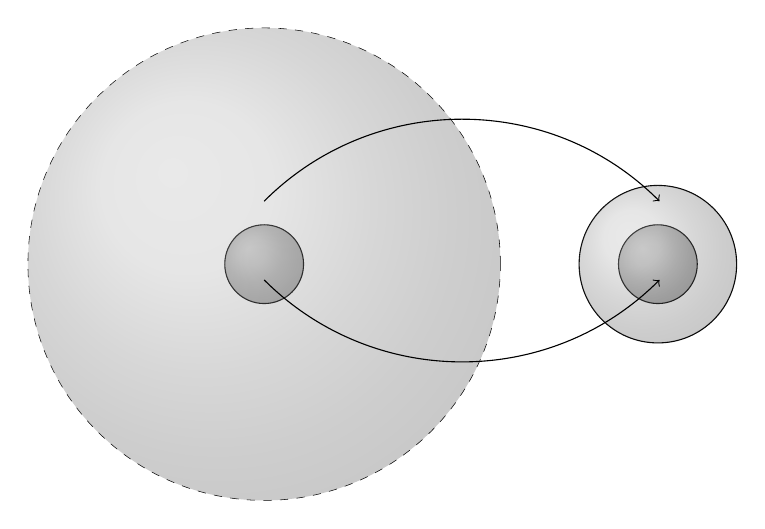
\begin{tikzpicture}
\filldraw[fill = black!10!white, draw = black, dashed, very thin] (0,0) circle (3);
\filldraw[fill = black!30!white, draw = black] (0,0) circle (0.5);
\filldraw[fill = black!10!white, draw = black] (5,0) circle (1.0);
\filldraw[fill = black!30!white, draw = black] (5,0) circle (0.5);
\shade[ball color=black!30!white,opacity=0.20] (0,0) circle (0.5);
\shade[ball color=black!10!white,opacity=0.20] (0,0) circle (3);
\shade[ball color=black!30!white,opacity=0.20] (5,0) circle (0.5);
\shade[ball color=black!10!white,opacity=0.20] (5,0) circle (1);
\draw[->] (0,-0.2) arc (225:315:3.55);
\draw[->] (0,0.8) arc (135:45:3.55);
\end{tikzpicture}
\end{figure}


La trasformazione viene progettata per lasciare inalterata la regione interna e modificare il dominio aperto che circonda la regione interna condensandolo nel volume finito della \textit{BR} (fig. \ref{fig:4.9}).

Esistono in letteratura molte varianti di trasformazione che si differenziano per il tipo di problema (2D, 3D), per la geometria delle regioni (prismatica, sferica, etc.) e per l'ordine. In \cite{brunotte_finite_1992} si sottolinea come non sia strettamente necessaria neppure la conformità stessa della trasformazione.

\subsection{Spherical Shell Transformation}

In questo lavoro è stata sviluppata una trasformazione radiale rispetto all'origine degli assi di ordine $\alpha$ regolabile, basata sulla progettazione circolare (2D) o sferica (3D) dei domini che chiameremo \textit{spherical shell transformation} (\textit{SST}). Queste caratteristiche permettono una certa elasticità nel suo utilizzo a scapito di una progettazione della geometria meno libera.

\begin{figure}[htp]
\centering
\caption{Domini della \textit{spherical shell transformation}}
\label{fig:4.10}
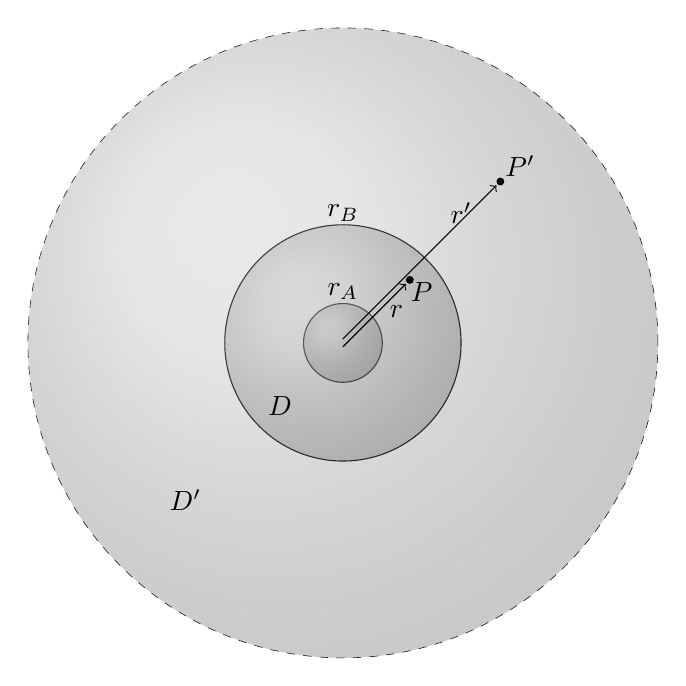
\begin{tikzpicture}
\filldraw[fill = black!10!white, draw = black, dashed, very thin] (0,0) circle (4);
\filldraw[fill = black!20!white, draw = black] (0,0) circle (1.5);
\filldraw[fill = black!30!white, draw = black] (0,0) circle (0.5);
\shade[ball color=black!30!white,opacity=0.20] (0,0) circle (0.5);
\shade[ball color=black!20!white,opacity=0.20] (0,0) circle (1.5);
\shade[ball color=black!10!white,opacity=0.20] (0,0) circle (4);
\fill[black] (2,2.05) circle (0.05);
\fill[black] (0.85,0.8) circle (0.05);
\draw[->] (0,0.05) -- (1.95,2.);
\draw[->] (0,-0.05) -- (.8,.75);
\draw (2.25, 2.25) node {$P'$}; %label
\draw (1, 0.65) node {$P$}; %label
\draw (1.5, 1.65) node {$r'$}; %label
\draw (0.68, 0.4) node {$r$}; %label
\draw (0,0.65) node {$r_A$}; %label
\draw (0,1.65) node {$r_B$}; %label
\draw (-2,-2) node {$\TTTT{D'}$}; %label
\draw (-.8,-.8) node {$\TTTT{D}$}; %label
\end{tikzpicture}
\end{figure}

Con riferimento alla figura \ref{fig:4.10} verrà chiamato con $P'\left(r',\vartheta', \varphi'\right)$ il punto appartenente alla regione aperta $\TTTT{D'}$ e con $P\left(r,\vartheta,\varphi\right)$ il punto appartenente alla \textit{boundary region} $\TTTT{D}$.

La mappa è così definita:
\begin{align}
\label{eq:4trans_a}
r'&=r_A \left(\frac{r_B-r_A}{r_B-r}\right)^\alpha \\
\label{eq:4trans_b}
r &= r_B -\left(r_B-r_A\right)\left(\frac{r_A}{r'}\right)^{\frac{1}{\alpha}},
\end{align}
dove $r_A$  e $r_B$ sono rispettivamente il raggio interno ed esterno della \textit{BR}.

Si possono osservare le seguenti proprietà:
\begin{aenumerate}
\item Il generico punto $P'$ viene proiettato lungo la direzione radiale in un punto appartenente al segmento $P_A-P_B$, in modo che $\vartheta' = \vartheta$, $\varphi' = \varphi$ e $r_A \leq r \leq r_B$;
\item Il punto $P'_A$ coincide con la sua proiezione $P_A$ per mantenere la continuità nella transizione tra la regione interna e la \textit{BR};
\item Per $\left\{r' \rightarrow \infty\right\}$  $P$ viene proiettato sul punto $P_B$, ossia sul raggio esterno della \textit{BR};
\item Un dato numero di punti della \textit{BR} (ad esempio i nodi della \textit{mesh}) rappresentano le immagini di punti tanto più lontani fra loro e distanti dall'origine quanto più alto è il parametro $\alpha$. 
\item Si può regolare il parametro $\alpha$ in modo da soddisfare la continuità delle derivate in direzione radiale nel passaggio dalla regione interna alla \textit{BR} imponendo la condizione:
\begin{align}
\label{eq:4derivata_continua}
\left[\frac{\partial r}{\partial r'}\right]_{r_A} &= 1\nonumber\\
\left[\frac{\left(r_B-r_A\right)\left(\frac{r_A}{r'}\right)^{\frac{1}{\alpha}}}{\alpha r'}\right]_{r_A} &= 1\nonumber\\
\frac{\left(r_B-r_A\right)}{\alpha r_A} &= 1,
\end{align}
da cui
\begin{equation}
\label{eq:4derivata_continua2}
\alpha = \frac{\left(r_B-r_A\right)}{r_A}.
\end{equation}
Questa condizione è stata riportata a titolo di completezza; tuttavia la continuità delle derivate in direzione radiale non è necessaria per una corretta applicazione del metodo. Pertanto il codice è stato sviluppato soltanto per ordini di decadimento $\alpha$ interi.
\end{aenumerate}

\subsection{Applicazione in 2D}

La trasformazione radiale deve essere ora applicata allo spazio cartesiano in cui viene definito il problema in forma debole.

Richiamiamo quindi la trasformazione che porta da coordinate cartesiane 2D $\left(x,y\right)$ a polari $\left(r,\vartheta\right)$.

\begin{equation}
\label{eq:4polare1}
\left\{
\begin{aligned}
x = r \cos \vartheta\\
y = r \sin\vartheta
\end{aligned}
\right. 
\qquad\qquad
\left\{
\begin{aligned}
r = \sqrt[]{x^2+y^2}\\
\vartheta = \arctan \frac{y}{x}
\end{aligned}
\right.
\end{equation}
\begin{align}
\label{eq:4polare2}
\left\{\begin{aligned}\partial x\\ \partial y\end{aligned}\right\}
&= \left[\begin{array}{cc}
\cos \vartheta & -r\sin \vartheta\\
\sin \vartheta & r\cos\vartheta\end{array}\right]
\left\{\begin{aligned}\partial r\\ \partial\vartheta\end{aligned}\right\}
=\left[T_{r\rightarrow x}\right]\left\{\begin{aligned}\partial r\\ \partial\vartheta\end{aligned}\right\}\\
\label{eq:4polare3}
\left\{\begin{aligned}\partial r\\ \partial\vartheta\end{aligned}\right\}
&= \left[\begin{array}{cc}
\cos \vartheta & \sin \vartheta\\
-\frac{\sin \vartheta}{r} & \frac{\cos\vartheta}{r}\end{array}\right]
\left\{\begin{aligned}\partial x\\ \partial y\end{aligned}\right\}
=\left[T_{x\rightarrow r}\right]\left\{\begin{aligned}\partial x\\ \partial y\end{aligned}\right\}
\end{align}
\begin{align}
\label{eq:4polare4_a}
\text{det}\left(\left[T_{r\rightarrow x}\right]\right) &= r\\
\label{eq:4polare4_b}
\text{det}\left(\left[T_{x\rightarrow r}\right]\right) &= \frac{1}{r}
\end{align}

Esprimiamo ora la \textit{SST} in forma matriciale in coordinate polari:
\begin{equation}
\label{eq:42dtrans}
\left\{\begin{aligned}\partial r' \\ \partial \vartheta' \end{aligned}\right\}
= \left[\begin{array}{cc}\frac{\partial r'}{\partial r} & 0\\0&1\end{array}\right]
\left\{\begin{aligned}\partial r \\ \partial \vartheta \end{aligned}	\right\} = \left[T_{r\rightarrow r'}\right]\left\{\begin{aligned}\partial r \\ \partial \vartheta \end{aligned}	\right\}.
\end{equation}

La trasformazione globale da $\T{x}$ a $\T{x'}$ si ottiene componendo le trasformazioni nell'ordine corretto:
\begin{equation}
\label{eq:4composizione1}
\T{x}\longrightarrow\T{r}\longrightarrow\T{r'}\longrightarrow\T{x'},
\end{equation}
ovvero
\begin{align}
\label{eq:4composizione2}
\left\{\begin{aligned}\partial x'\\ \partial y'\end{aligned}\right\} &= \left[T_{r'\rightarrow x'}\right] \left\{\begin{aligned}\partial r'\\ \partial \vartheta'\end{aligned}\right\}\nonumber\\
&=\left[T_{r'\rightarrow x'}\right] \left[T_{r\rightarrow r'}\right]\left\{\begin{aligned}\partial r\\ \partial \vartheta\end{aligned}\right\}\nonumber\\
&=\left[T_{r'\rightarrow x'}\right] \left[T_{r\rightarrow r'}\right]\left[T_{x\rightarrow r}\right]\left\{\begin{aligned}\partial x\\ \partial y\end{aligned}\right\}\nonumber\\
&=\left[T_{x \rightarrow x'}\right]\left\{\begin{aligned}\partial x\\ \partial y\end{aligned}\right\},
\end{align}

ed eseguendo i prodotti si ottiene:
\begin{equation}
\label{eq:4composizione3}
\left[T_{x\rightarrow x'}\right]=
\left[\begin{array}{cc}
\frac{\partial r'}{\partial r}\cos^2 \vartheta+\frac{r'}{r}\sin^2\vartheta &
\cos\vartheta \sin\vartheta\left(\frac{\partial r'}{\partial r}-\frac{r'}{r}\right)\\
\cos\vartheta\sin\vartheta\left(\frac{\partial r'}{\partial r}-\frac{r'}{r}\right) & \frac{\partial r'}{\partial r}\sin^2 \vartheta+\frac{r'}{r}\cos^2\vartheta
\end{array}\right],
\end{equation}
\begin{align}
\label{eq:4composizione3_bis}
\frac{\partial x'}{\partial x} &= \frac{\partial r'}{\partial r}\cos^2 \vartheta+\frac{r'}{r}\sin^2\vartheta,\nonumber\\
\frac{\partial x'}{\partial y} &= \frac{\partial y'}{\partial x} =
\cos\vartheta \sin\vartheta\left(\frac{\partial r'}{\partial r}-\frac{r'}{r}\right),\nonumber\\
\frac{\partial y'}{\partial y}&=\frac{\partial r'}{\partial r}\sin^2 \vartheta+\frac{r'}{r}\cos^2\vartheta.\nonumber
\end{align}
\begin{equation}
\label{eq:4det2d}
\text{det}\left(\left[ T_{x\rightarrow x'} \right] \right)=\frac{\partial r'}{\partial r}\frac{r'}{r}
\end{equation}

Descriviamo ora gli operatori differenziali in funzione delle coordinate del dominio trasformato; si inizi con il gradiente di uno scalare:
\begin{align}
\label{eq:4boundarygrad2d}
\grad'\left(u\right) &= \left\{
\begin{array}{c}
\frac{\partial u}{\partial x'}\\
\frac{\partial u}{\partial y'}
\end{array}
\right\} = \left\{
\begin{array}{c}
\frac{\partial u}{\partial x} \frac{\partial x}{\partial x'}+\frac{\partial u}{\partial y} \frac{\partial y}{\partial x'}\\
\frac{\partial u}{\partial x} \frac{\partial x}{\partial y'}+\frac{\partial u}{\partial y} \frac{\partial y}{\partial y'}\end{array}\right\}
 =\nonumber\\
&=  \left[
\begin{array}{cc}
\frac{\partial x}{\partial x'} & \frac{\partial y}{\partial x'}\\
\frac{\partial x}{\partial y'} & \frac{\partial y}{\partial y'}
\end{array}
\right]
\left\{
\begin{array}{c}
\frac{\partial u}{\partial x}\\
\frac{\partial u}{\partial y}
\end{array}
\right\}= \TT{J}^{-1} \cdot \grad\left(u\right).
\end{align}

Si prosegua ora con il rotore di uno scalare:
\begin{align}
\label{eq:4boundaryrot2d}
\rot'\left(u\right) &= \left\{
\begin{array}{c}
\;\frac{\de u}{\de y'}\\
-\frac{\de u}{\de x'}
\end{array}
\right\} = \nonumber \\
&=\left\{
\begin{array}{c}
\frac{\de u}{\de x} \frac{\de x}{\de y'}+\frac{\de u}{\de y} \frac{\de y}{\de y'}\\
-\frac{\de u}{\de x} \frac{\de x}{\de y'}-\frac{\de u_x}{\de y} \frac{\de y}{\de y'}
\end{array}\right\}
\end{align}

Infine, si calcoli il termine $dv' = dx' \cdot dy'$:
\begin{equation}
\label{2boundaryjacobian2d}
dv' = dx' \cdot dy'= \text{det}\left(\TT{J}\right)\cdot dx \cdot dy=  \text{det}\left(\TT{J}\right) dv
\end{equation}

\subsection{Applicazione in 3D}
Analogamente, cerchiamo la \textit{SST} per il problema tridimensionale.
Introducendo i sistemi di coordinate $\T{x}=\left\{x, y, z\right\}^T$ e $\T{r}=\left\{r, \vartheta, \varphi\right\}^T$ abbiamo:


\begin{equation}
\label{eq:4sferiche1}
\left\{
\begin{aligned}
x &= r \cos \vartheta\sin\varphi\\
y &= r \sin\vartheta\sin\varphi\\
z &= r \cos \varphi
\end{aligned}
\right. 
\qquad\qquad
\left\{
\begin{aligned}
r &= \sqrt[]{x^2+y^2+z^2}\\
\vartheta &= \arctan \frac{y}{x}\\
\varphi &= \arccos\frac{z}{r}
\end{aligned}
\right.
\end{equation}
\begin{align}
\label{eq:4sferiche2}
\left\{\begin{aligned}\partial x\\ \partial y\\ \partial z\end{aligned}\right\}
&= \left[\begin{array}{ccc}
\cos \vartheta\sin\varphi &-r\sin\vartheta\sin\varphi & r\cos\vartheta\cos\varphi\\
\sin \vartheta\sin\varphi & r\cos\vartheta\sin\varphi & r\sin\vartheta\cos\varphi\\
\cos\varphi & 0 & -r\sin\varphi\end{array}\right]
\left\{\begin{aligned}\partial r\\ \partial\vartheta\\ \partial\varphi\end{aligned}\right\}\\
\label{eq:4sferiche3}
\left\{\begin{aligned}\partial r\\ \partial\vartheta\\ \partial\varphi\end{aligned}\right\}
&= \left[\begin{array}{ccc}
\cos \vartheta\sin\varphi &\sin\vartheta\sin\varphi & \cos\varphi\\
-\frac{\sin \vartheta}{r\sin\varphi} & \frac{cos\vartheta}{r\sin\varphi} & 0\\
\frac{\cos\vartheta\cos\varphi}{r} & \frac{\sin\vartheta\cos\varphi}{r} & -\frac{\sin\varphi}{r}\end{array}\right]
\left\{\begin{aligned}\partial x\\ \partial y\\ \partial z\end{aligned}\right\}
\end{align}
\begin{align}
\label{eq:4sferiche4_a}
det\left(\left[T_{r\rightarrow x}\right]\right) &= r^2 \sin\varphi\\
\label{eq:4sferiche4_b}
det\left(\left[T_{x\rightarrow r}\right]\right) &= \frac{1}{r^2\sin\varphi}.
\end{align}

Scrivendo la \textit{SST} in coordinate sferiche:
\begin{equation}
\label{eq:43dtrans}
\left\{\begin{aligned}\partial r' \\ \partial \vartheta' \\ \partial\varphi'\end{aligned}\right\}
= \left[\begin{array}{ccc}\frac{\partial r'}{\partial r} & 0 & 0\\ 0&1&0\\0&0&1\end{array}\right]
\left\{\begin{aligned}\partial r \\ \partial \vartheta\\ \partial\varphi \end{aligned}	\right\} = \left[T_{r\rightarrow r'}\right]\left\{\begin{aligned}\partial r \\ \partial \vartheta \\ \partial\varphi\end{aligned}	\right\}.
\end{equation}

Infine, si compongono le trasformazioni:

\begin{align}
\label{eq:4composizione4}
\left\{\begin{aligned}\partial x'\\ \partial y'\\ \partial z'\end{aligned}\right\} &=\left[T_{r'\rightarrow x'}\right] \left[T_{r\rightarrow r'}\right]\left[T_{x\rightarrow r}\right]\left\{\begin{aligned}\partial x\\ \partial y\\ \partial z\end{aligned}\right\}\nonumber\\
&=\left[T_{x \rightarrow x'}\right]\left\{\begin{aligned}\partial x\\ \partial y\\ \partial z\end{aligned}\right\}.
\end{align}

Ancora, eseguendo i prodotti:
\begin{align}
\label{eq:4composizione5}
\frac{\partial x'}{\partial x} &= \frac{\partial r'}{\partial r}\cos^2 \vartheta\sin^2\varphi+\frac{r'}{r}\left(\sin^2\vartheta+\cos^2 \vartheta\cos^2\varphi\right),\nonumber\\
\frac{\partial x'}{\partial y} &= \frac{\partial y'}{\partial x} =
\sin\vartheta\cos\vartheta\left[\frac{\partial r'}{\partial r}\sin^2\varphi+\frac{r'}{r}\left(cos^2\varphi-1\right)\right] 
,\nonumber\\
\frac{\partial x'}{\partial z}&=\frac{\partial z'}{\partial x}=\cos\vartheta \sin\varphi\cos\varphi\left(\frac{\partial r'}{\partial r}-\frac{r'}{r}\right),\nonumber\\
\frac{\partial y'}{\partial y}&=\frac{\partial r'}{\partial r}\sin^2 \vartheta\sin^2\varphi+\frac{r'}{r}\left(\cos^2\vartheta+\sin^2 \vartheta\cos^2\varphi\right),\nonumber\\
\frac{\partial y'}{\partial z} &= \frac{\partial z'}{\partial y} = \cos\vartheta \sin\varphi\cos\varphi\left(\frac{\partial r'}{\partial r}-\frac{r'}{r}\right),\nonumber\\
\frac{\partial z'}{\partial z} &= \frac{\partial r'}{\partial r}\cos^2\varphi+\frac{r'}{r}\sin^2\varphi.\nonumber
\end{align}
\begin{equation}
\label{eq:4det2d_bis}
\text{det}\left(\left[T_{x\rightarrow x'}\right]\right)=\frac{\partial r'}{\partial r}\left(\frac{r'}{r}\right)^2
\end{equation}

Descriviamo ora gli operatori differenziali in funzione delle coordinate del dominio trasformato; si inizi con il gradiente di uno scalare:
\begin{align}
\label{eq:4boundarygrad2d_bis}
\grad'\left(u\right) &= \left\{
\begin{array}{c}
\frac{\partial u}{\partial x'}\\
\frac{\partial u}{\partial y'}\\
\frac{\partial u}{\partial z'}
\end{array}
\right\} = \left\{
\begin{array}{c}
\frac{\partial u}{\partial x} \frac{\partial x}{\partial x'}+\frac{\partial u}{\partial y} \frac{\partial y}{\partial x'}+\frac{\partial u}{\partial z} \frac{\partial z}{\partial x'}\\
\frac{\partial u}{\partial x} \frac{\partial x}{\partial y'}+\frac{\partial u}{\partial y} \frac{\partial y}{\partial y'}+\frac{\partial u}{\partial z} \frac{\partial z}{\partial y'}\\
\frac{\partial u}{\partial x} \frac{\partial x}{\partial z'}+\frac{\partial u}{\partial y} \frac{\partial y}{\partial z'}+\frac{\partial u}{\partial z} \frac{\partial z}{\partial z'}
\end{array}\right\} =\nonumber\\
&=  \left[
\begin{array}{ccc}
\frac{\partial x}{\partial x'} & \frac{\partial y}{\partial x'} & \frac{\partial z}{\partial x'}\\
\frac{\partial x}{\partial y'} & \frac{\partial y}{\partial y'} & \frac{\partial z}{\partial y'}\\
\frac{\partial x}{\partial z'} & \frac{\partial y}{\partial z'} & \frac{\partial z}{\partial z'}
\end{array}
\right]
\left\{
\begin{array}{c}
\frac{\partial u}{\partial x}\\
\frac{\partial u}{\partial y}\\
\frac{\partial u}{\partial z}
\end{array}
\right\}= \TT{J}^{-1} \cdot \grad\left(u\right).
\end{align}

Si prosegua ora con il rotore:
\begin{align}
\label{eq:4boundaryrot2d_bis}
\rot'\left(\T{u}\right) &= \left\{
\begin{array}{c}
\frac{\de u_z}{\de y'}-\frac{\de u_y}{\de z'}\\
\frac{\de u_x}{\de z'}-\frac{\de u_z}{\de x'}\\
\frac{\de u_y}{\de x'}-\frac{\de u_x}{\de y'}\\
\end{array}
\right\} = \nonumber \\
&=\left\{
\begin{array}{c}
\frac{\de u_z}{\de x} \frac{\de x}{\de y'}+\frac{\de u_z}{\de y} \frac{\de y}{\de y'}+\frac{\de u_z}{\de z} \frac{\de z}{\de y'}\\
\frac{\de u_x}{\de x} \frac{\de x}{\de z'}+\frac{\de u_x}{\de y} \frac{\de y}{\de z'}+\frac{\de u_x}{\de z} \frac{\de z}{\de z'}\\
\frac{\de u_y}{\de x} \frac{\de x}{\de x'}+\frac{\de u_y}{\de y} \frac{\de y}{\de x'}+\frac{\de u_y}{\de z} \frac{\de z}{\de x'}
\end{array}\right\}+\nonumber\\
&-\left\{
\begin{array}{c}
\frac{\de u_y}{\de x} \frac{\de x}{\de z'}+\frac{\de u_y}{\de y} \frac{\de y}{\de z'}+\frac{\de u_y}{\de z} \frac{\de z}{\de z'}\\
\frac{\de u_z}{\de x} \frac{\de x}{\de x'}+\frac{\de u_z}{\de y} \frac{\de y}{\de x'}+\frac{\de u_z}{\de z} \frac{\de z}{\de x'}\\
\frac{\de u_x}{\de x} \frac{\de x}{\de y'}+\frac{\de u_x}{\de y} \frac{\de y}{\de y'}+\frac{\de u_x}{\de z} \frac{\de z}{\de y'}
\end{array}
\right\}
\end{align}

Infine, si calcoli il termine $dv' = dx' \cdot dy' \cdot dz'$:
\begin{equation}
\label{4boundaryjacobian2d_bis}
dv' = dx' \cdot dy' \cdot dz' = \text{det}\left(\TT{J}\right)\cdot dx \cdot dy \cdot dz =  \text{det}\left(\TT{J}\right) dv
\end{equation}


\section{Test-case: due fili in 2D}
\label{subsec:2fili}
Verranno qui mostrati i risultati ottenuti confrontando l'andamento del campo di induzione magnetica generato da due superfici cilindriche di lunghezza indefinita lungo le quali scorre in direzione assiale una corrente superficiale uguale e concorde. La geometria del modello è riassunta in Tabella \ref{tab:fili2d}, mentre la soluzione in termini di campo $\T{b}$ è mostrata in Figura \ref{fig:SR_2D_tris}. \'E stato scelto un problema bidimensionale in cui il decadimento è lento ($\frac{1}{r}$). In questo modo è possibile rilevare meglio il contributo dell'applicazione della SST nella simulazione di problemi aperti. In 3D il decadimento dei campi è sicuramente più rapido e l'effetto della trasformazione è minore e meno evidente. Tuttavia se l'obiettivo dell'analisi è il calcolo di forze magnetiche o induttanze, è importante rilevare che la loro sensibilità rispetto ai valori assunti dal campo elettro-magnetico anche lontano dai corpi è alta. Pertanto l'utilizzo della SST è stato utilizzato in tutte le analisi successive, sia bidimensionali che tridimensionali.

\begin{table}[hb]
\caption{Dati geometrici utilizzati per il caso test}
\label{tab:fili2d}
\centering
\begin{tabular}{lcc}
\toprule
Raggio fili & $r$ & 0.35 m\\
Distanza fili &$d$ & 5 m\\
Raggio interno BR &$r_a$ & 10 m\\
Raggio esterno BR &$r_b$ & 15 m\\
\bottomrule
\end{tabular}
\end{table}

\begin{figure}[htb]
    \centering
    
\includegraphics[width = .6\textwidth]{SR_2D_tris}
    \caption{Linee di flusso della soluzione al \textit{test case} per la BR in 2D}
    \label{fig:SR_2D_tris}
\end{figure}

In Figura \ref{fig:SR_2D} è mostrato l'andamento del campo, confrontando l'analisi senza BR  (caso \textit{a}) con quelle effettuate attivando la BR; per evidenziare la variazione di intensità di campo è mostrato il caso con ordine di decadimento $\alpha = 3$.
 
\begin{figure}
    \centering
    \subfloat[][]{
\includegraphics[width = .45\textwidth]{SR_2D_a}\label{SR_2D_a}}\quad
    \subfloat[][]{
\includegraphics[width = .45\textwidth]{SR_2D_b3}\label{SR_2D_b3}}
    \caption{Confronto fra le induzioni magnetiche generate  senza e con l'attivazione della BR di ordine 3}
     \label{fig:SR_2D}
\end{figure}


Si può notare, grazie al confronto in Figura \ref{fig:SR_2D_bis} che mostra il modulo dell'induzione magnetica in funzione della distanza dal punto centrale, che il decadimento del campo magnetico viene correttamente rappresentato solo con l'attivazione del metodo.  

Si riporta che l'andamento teorico mostrato in figura è scalato di un fattore pari a 1.04 poiché, mentre nel caso ideale la corrente totale che attraversa i fili è pari a $2\pi r\T{j}$, la corrente totale nelle analisi numeriche è data da $2p\T{j}$, dove $2p$ è il perimetro effettivo della mesh che riproduce la circonferenza. Il fattore di scalatura riportato è stato ottenuto stimando il numero di lati del poligono circoscritto alla circonferenza con lato pari alla dimensione media degli elementi nella zona considerata.

Si osservi l'andamento del grafico nella zona della BR: con il primo ordine il campo assume un andamento lineare e negli altri casi l'abbattimento è più marcato. 

Si noti inoltre che i tre casi di applicazione del metodo danno curve coincidenti nella regione interna.
\begin{landscape}
\begin{figure}[htb]
   \centering
    \begin{tikzpicture}
    \begin{axis}[axis y line = left,
                 axis x line = left,
    		     xmin = 0,
    		     width = 1.5\textwidth,
    		     height = \textheight,
                 xlabel = {$r$ (m)}, 
                 ylabel = {$\T{b}$ (T)}]
    \addplot[black, samples = 200, smooth]
    file {./Immagini/Boundary/SR_2Dteorico.dat};
    \addplot[black!60!white, thick, dotted, samples = 100, smooth]
    file {./Immagini/Boundary/SR_2D_0.dat};
    \addplot[red,dashed, samples = 200, smooth]
    file {./Immagini/Boundary/SR_2D_1.dat};
    \addplot[green,dashed, samples = 100, smooth]
    file {./Immagini/Boundary/SR_2D_2.dat};
    \addplot[blue,dashed, samples = 200, smooth]
    file {./Immagini/Boundary/SR_2D_3.dat};
    \legend{$Teoric$\\$No~SST$\\$\alpha = 1$\\$\alpha = 2$\\$\alpha=3$\\}
    \draw[red,  thick] (10,0)-- (10,0.1);
    \end{axis}
    \end{tikzpicture}
    \caption{Confronto del decadimento del campo $\T{b}$ nel caso bidimensionale}
    \label{fig:SR_2D_bis}
\end{figure}
\end{landscape}




\section{Regioni conduttive in regime quasi-stazionario}

Questa sezione riassume le considerazioni fatte sull'effetto della variazione nel tempo del flusso di un campo magnetico in una regione conduttiva. La variazione di $\Phi(\T{b})$ causa la nascita di un campo elettrico all'interno del conduttore; il comportamento del materiale dipende dalla conducibilità del materiale e dalla frequenza di variazione del campo magnetico\ \citep{haus_electromagnetic_1989}.


Se la variazione di flusso è rapida (ad alta frequenza) domina il comportamento induttivo del materiale conduttore: il campo elettrico indotto provoca la nascita di correnti di spostamento $\T{j}$ che inducono a loro volta un campo magnetico. Questo si sovrappone con il campo esterno in modo da annullarlo all'interno del dominio. In questo caso si può riassumere il comportamento della regione imponendo la non-penetrazione del campo magnetico all'interno della regione conduttiva. Infatti il materiale si scherma dal campo generando delle correnti in prossimità della superficie nello stesso modo in cui si scherma dal campo elettrico generando una distribuzione di cariche superficiali. Possiamo quindi scrivere: 
\begin{equation}
\label{eq:4cond1}
\T{b}\cdot \T{n} = 0.
\end{equation}

La corrente indotta (superficiale) può essere espressa come:
\begin{equation}
\label{eq:4cond2}
\T{j_{s}} = -\T{h}\times\T{n},
\end{equation}

Se, al contrario, la variazione di flusso è lenta (a bassa frequenza) il campo elettrico indotto è troppo basso per generare un'interferenza magnetica; il conduttore è inerte e può essere trattato solamente tramite le sue proprietà magnetiche. 
In questo secondo caso, quindi, la presenza del materiale conduttore non altera le condizioni al contorno del problema magnetico. Il materiale è dominato dalle sue proprietà resistive e la corrente indotta (volumetrica) può essere calcolata a posteriori:
\begin{equation}
\label{eq:4cond3}
\T{j} = \sigma\T{e} = \sigma~\de_t\T{a}.
\end{equation}
Nella situazione intermedia la dinamica dello sviluppo delle correnti non può essere trascurata e il campo magnetico ed elettrico tornano ad essere dipendenti l'uno dall'altro, non per l'accoppiamento dinamico proprio delle equazioni di Maxwell bensì per la natura del legame costitutivo. Le analisi vengono in questi casi effettuate risolvendo equazioni di diffusione.

Poiché nel caso dell'ottica adattiva i sensori capacitivi e gli attuatori induttivi sono co-locati (e quindi molto vicini) e le frequenze di controllo sono elevate (fino a $10^5$ Hz)  è necessaria un'analisi preliminare per una stima dell'ordine di grandezza delle correnti indotte nel condensatore a causa del movimento relativo tra questo e gli elementi dell'attuatore. In questo esempio la variazione di flusso è generata dalla corrente variabile nell'induttore, ma lo stesso principio vale anche nel caso di parti in movimento relativo. In quest'ottica è stata scelta come rappresentativa la frequenza di $100$ kHz, nell'ipotesi che per frequenze maggiori l'ampiezza del movimento dello specchio sia trascurabile.

Dato che i coating metallici che compongono le armature del condensatore hanno lo spessore di pochi micron, l'analisi sarà ristretta a conduttori sottili modellabili attraverso semplici superfici conduttive.

\tikzset{
  pics/.cd,
  disc/.style = {
    code = {
      \fill [white] ellipse [x radius = 2, y radius = 2/3];
      \path [left color = black!50, right color = black!50,
        middle color = black!25] 
        (-2+.05,-1.1) arc (180:360:2-.05 and 2/3-.05*2/3) -- cycle;
      \path [top color = black!25, bottom color = white] 
        (0,.05*2/3) ellipse [x radius = 2-.05, y radius = 2/3-.05*2/3];
      \path [left color = black!25, right color = black!25,
        middle color = white] (-2,0) -- (-2,-1) arc (180:360:2 and 2/3)
        -- (2,0) arc (360:180:2 and 2/3);
      \foreach \r in {225,315}
        \foreach \i [evaluate = {\s=30;}] in {0,2,...,30}
          \fill [black, fill opacity = 1/50] 
            (0,0) -- (\r+\s-\i:2 and 2/3) -- ++(0,-1) 
            arc (\r+\s-\i:\r-\s+\i:2 and 2/3) -- ++(0,1) -- cycle;
      \foreach \r in {45,135}
        \foreach \i [evaluate = {\s=30;}] in {0,2,...,30}
          \fill [black, fill opacity = 1/50] 
            (0,0) -- (\r+\s-\i:2 and 2/3) 
            arc (\r+\s-\i:\r-\s+\i:2 and 2/3)  -- cycle;
    }
  },
  disc2/.style = {
    code = {
      \fill [white] ellipse [x radius = 2, y radius = 2/3];
      \path [top color = black!25, bottom color = white] 
        (0,.05*2/3) ellipse [x radius = 2-.05, y radius = 2/3-.05*2/3];
      \path [left color = black!25, right color = black!25,
        middle color = white] (-2,0) -- (-2,-.01) arc (180:360:2 and 2/3)
        -- (2,0) arc (360:180:2 and 2/3);
      \foreach \r in {225,315}
        \foreach \i [evaluate = {\s=30;}] in {0,2,...,30}
          \fill [black, fill opacity = 1/50] 
            (0,0) -- (\r+\s-\i:2 and 2/3) -- ++(0,-.01)
            arc (\r+\s-\i:\r-\s+\i:2 and 2/3) -- ++(0,.01)-- cycle;
      \foreach \r in {45,135}
        \foreach \i [evaluate = {\s=30;}] in {0,2,...,30}
          \fill [black, fill opacity = 1/50] 
            (0,0) -- (\r+\s-\i:2 and 2/3) 
            arc (\r+\s-\i:\r-\s+\i:2 and 2/3)  -- cycle;
    }
  }
}
\begin{SCfigure}[1.5][htb]
\centering
\caption{Esempio di analisi di diffusione: piastra metallica posta a breve distanza da un solenoide}
\label{fig:4cond_ind_example}
\tdplotsetmaincoords{55}{45}
\resizebox{.3\textwidth}{!}{
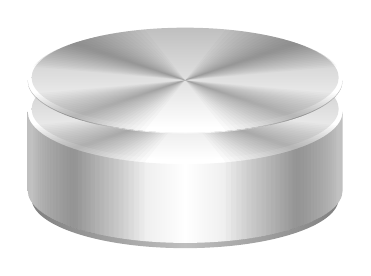
\begin{tikzpicture}
\path (0,0) pic {disc} (0,0.4) pic {disc2};
\end{tikzpicture}}
\end{SCfigure}


Si prenda in considerazione il sistema mostrato in Figura \ref{fig:4cond_ind_example} composto da una piastra metallica sottile posta su un induttore solenoidale.

Si supponga per semplicità che il solenoide generi un campo $\T{h}$ armonico con periodo $T$ che in prossimità della piastra sia costante e normale alla superficie. Considerando una circonferenza di raggio $r<R$ interna al disco si ha allora:
\begin{equation}
\label{eq:4es1}
2\pi r e = \mu \pi r^2 \de_t h,
\end{equation}
da cui
\begin{equation}
\label{eq:4es2}
e = \mu \frac{r}{2} \de_t h.
\end{equation}

Se la piastra possiede uno spessore $t$, scriviamo la corrente superficiale equivalente:

\begin{equation}
\label{eq:4es3}
j_s = \sigma e t = \mu \sigma \frac{r}{2} t \de_t h.
\end{equation}

\begin{table}
\centering
\caption{Dati ipotizzzati per la stima dell'entità del campo indotto su un sensore capacitivo} \label{tab:4daties}
\begin{tabular}{lc}
\toprule
Tipo sensore & Coating aureo\\
\midrule
Spessore & $1~\mu\text{m}$\\
Raggio & $10^-2$ m\\
Conduttività & $4.2553191~10^7 \frac{1}{\Omega\text{m}}$\\
Frequenza di controllo & $10^5 \text{Hz}$\\
\bottomrule
\end{tabular}
\end{table}
Si può ora stimare l'entità del campo magnetico indotto, approssimando l'integrale della corrente superficiale (che cresce linearmente con $r$) con il prodotto del raggio medio $R/2$ e della corrente corrispondente $j_s(R/2)$:
\begin{align}
\label{eq:4es4}
2\pi \frac{R}{2} h_{ind} &= i_{enc} = \int_0^R j_s(\chi) d\chi \approx \frac{R}{2} j_s (\frac{R}{2})\\
\label{eq:4es5}
h_{ind} &\approx\frac{\frac{R}{2} j_s (\frac{R}{2})}{2\pi \frac{R}{2}} = \frac{j_s(\frac{R}{2})}{2 \pi}.
\end{align}

Ne consegue un campo indotto medio pari a:
\begin{equation}
\label{eq:4es6}
h_{ind} \approx \mu \frac{ \sigma R t}{8\pi} \de_t h,
\end{equation}
da cui si ottiene un rapporto fra il campo generato dal solenoide $h$ e il campo indotto $h_{ind}$:
\begin{equation}
\label{eq:4es6bis}
\frac{h_{ind}}{h} \approx \mu \frac{ \sigma R t}{8\pi} \frac{\de_t h}{h} = \mu \frac{ \sigma R t}{8\pi} \omega = \mu \frac{ \sigma R t}{4T}.
\end{equation}

Si applichi la formula appena ottenuta supponendo dimensioni e frequenze compatibili con i sistemi applicati per l'ottica adattiva (Tabella \ref{tab:4daties}). Si ha:
\begin{equation}
\label{eq:4es7}
\frac{h_{ind}}{h}\approx 0.02
\end{equation}

Tale valore, ottenuto con ipotesi conservative (campo magnetico perpendicolare alla superficie conduttiva, stime pessimistiche dell'ordine di grandezza) suggerisce un comportamento del conduttore dominato dalle sue caratteristiche resistive. Questo legittima l'ipotesi dell'indipendenza del campo magnetico relativo agli attuatori dalla presenza dei sensori capacitivi. 
